\section{Experimental Simulation}
\label{simulation}

In this section, we describe a preliminary evaluation of the performance of an AMS for defending a substation against false data injection. We used a model of 1-generator 4-bus distribution system shown in Figure \ref{fig:example} (adopted from \cite{law2012security}) as the testbed, and compared the AMS's performance with that of the NE strategy proposed in \cite{law2012security,ma2013markov}. In this distribution system, the generator supplies electric power to four loads, and one STATCOM, connected to the system through Bus 3 (B3), regulates the voltage level by injecting (absorbing) reactive power to the system based on voltage feedback.
% As discussed in Section \ref{threatmodel}, the attacker intrudes the system and sends false voltage information back to the STATCOM, which might result in under-voltage and, eventually, load shedding. For the defender to protect against this kind of attack, certain detection algorithm can be implemented on the side of the STATCOM and the meter will be disconnected from the STATCOM if it detects that the meter has been compromised.

\begin{figure*}[t]
\setlength{\belowcaptionskip}{-12pt}
  \centering
\captionsetup[subfigure]{aboveskip=-1pt,belowskip=-7pt}~\hspace{-6em}
 \begin{subfigure}[b]{0.3\textwidth}
   \centering
                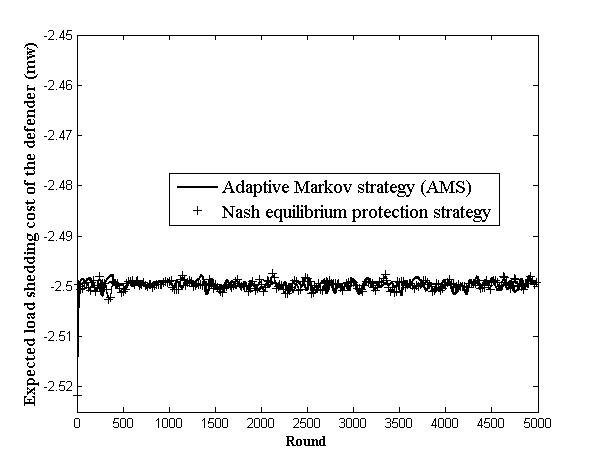
\includegraphics[width=1.4in]{result2}
                \caption{$\phi_0$: the NE strategy}
                \label{fig:NE}
        \end{subfigure}~\hspace{-6em}
 \begin{subfigure}[b]{0.3\textwidth}
   \centering
                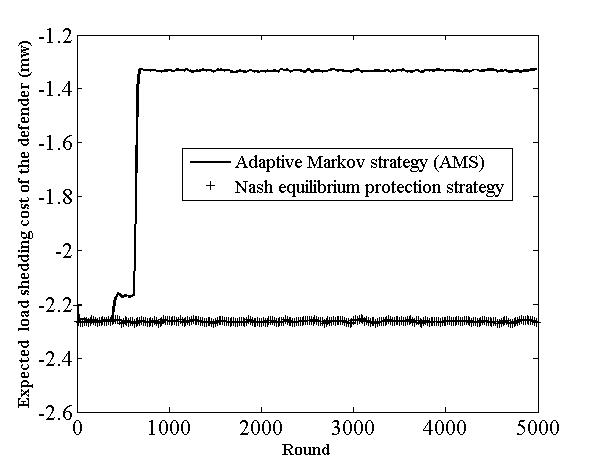
\includegraphics[width=1.4in]{result1}
                \caption{$\phi_1(s_1)  = \phi_1(s_2) = a _1$}
                \label{fig:a1}
        \end{subfigure}~\hspace{-6em}
\begin{subfigure}[b]{0.3\textwidth}
  \centering
                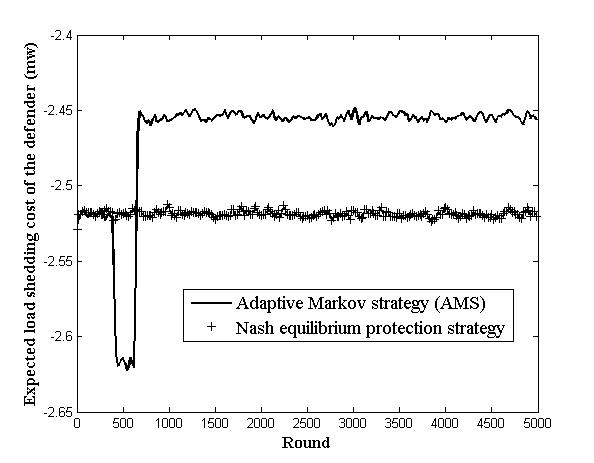
\includegraphics[width=1.4in]{result3}
                \caption{$\phi_2(s_1)  = \phi_2(s_2) = a _2$}
                \label{fig:a2}
        \end{subfigure}~\hspace{-4em}
\begin{subfigure}[b]{0.3\textwidth}
  \centering
                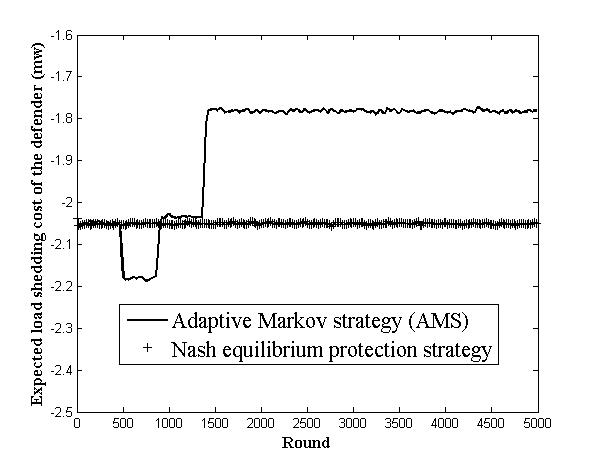
\includegraphics[width=1.4in]{result4}
                \caption{$\phi_3$: choose $a_1/a_2$ randomly}
                \label{fig:a1a2}
        \end{subfigure}~\hspace{-3em}
\begin{subfigure}[b]{0.3\textwidth}
  \centering
                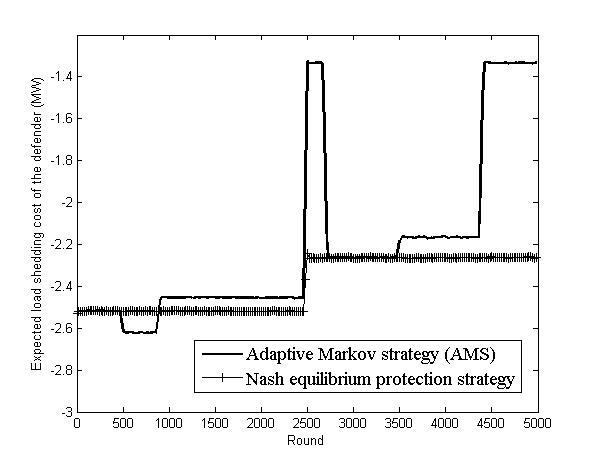
\includegraphics[width=1.4in]{result5}
                \caption{0 - 2500:$\phi_2$, 2500 - 5000: $\phi_1$}
                \label{fig:a2a1}
        \end{subfigure}
  \caption{\scriptsize{Expected load shedding cost of the system when the attacker employs different attacking strategies.}}
  \label{fig:games} %% label for entire figure
\end{figure*}

For our experiment, we constructed a Markov game based on the one used in the previous study of the false data injection attack \cite{law2012security}. In this game, the state space is abstracted into a set $S$ of two states, $S=\{s_1, s_2\}$, where $s_1$ and $s_2$ represent the states in which the system experiences (1) no load shedding, and (2) some amount of load shedding, respectively. The defender's action set is represented by $A_d = \{\tau_1 = 11,\tau_2 = 32\}$, which correspond to the two thresholds that the defender use to detect an injection attack. The attacker's action set is denoted by $A_a =\{k_1 = 1.1, k_2 = -0.8\}$, which correspond to two false voltage values that the attacker may choose to inject into the STATCOM. The transition probabilities and the expected immediate payoff of the defender  (the amount of load shedding that it prevents) for each joint action are obtained through Simulink \cite{dabney2001mastering} simulation and are shown as follows:
\[ Pr(d_1,a_1) = \left| \begin{array}{cc}
 43/45 & 2/45  \\
 1/2 & 1/2  \\ \end{array} \right|
 Pr(d_2,a_1) = \left| \begin{array}{cc}
 0 & 1  \\
 1/47 & 46/47  \\ \end{array} \right|\]

\[ Pr(d_1,a_2) = \left| \begin{array}{cc}
 48/49 & 1/49  \\
 0 & 1  \\ \end{array} \right|
 Pr(d_2,a_2) = \left| \begin{array}{cc}
 25/32 & 7/32\\
 7/17 & 10/17  \\ \end{array} \right|\]

\[ R_d(s_1) = \left| \begin{array}{cc}
 44/46 & 0  \\
 42/49 & 24/33  \\ \end{array} \right|
 R_d(s_2) = \left| \begin{array}{cc}
 2 & 2.50  \\
 2 & 2.15  \\ \end{array} \right|\]
We omit the details of the construction of the Markov game (including the suitability of the values in actions) since this is not the focus of our paper; interested readers may refer to \cite{law2012security} for details.

To evaluate the effectiveness of the AMS, we compare the performance of both the AMS and NE defending strategy under different attacker's strategies. We considered four different scenarios, where the attacker employs (1) a NE strategy, (2) a strategy where the attacker always performs $a_1$, (3) an $a_2$-only strategy, and (4) a random strategy. In each scenario, we ran a simulation of the Markov game for 5000 rounds, and measured the expected load sharing costs of the defender when it employed the AMS and NE strategy.

Figure \ref{fig:NE} shows the expected load shedding costs when the attacker selects the NE strategy. We can see that both defending strategies result in roughly the same load shedding cost. This is as expected; recognizing that the attacker is employing the NE strategy, the AMS learns to employ its optimal counterpart NE strategy for the defender.

Figure \ref{fig:a1} shows the expected load shedding costs when the attacker employs a strategy $\phi_1$ where he or she always performs the single action $a_1$. We can observe that the system's load shedding cost of the system is significantly reduced when the system employs the AMS. Intuitively, when the AMS recognizes that the attacker uses such a simple strategy, it also constructs an optimal strategy that exploits the attack pattern, thus minimizing the load shedding cost. Similarly, if the attacker employs the strategy $\phi_2$ where he always selects $a_2$ (Figure \ref{fig:a2}), the AMS constructs a corresponding optimal strategy that results in a significantly reduced cost over the NE strategy. The temporary drop-off around the 500th round is due to the fact that before the AMS can determine to an accurate estimation of the attacker's strategy, it may temporarily employ a strategy that is less than optimal. 

Figure \ref{fig:a1a2} illustrates the the load shedding costs when the attacker employs the strategy $\phi_3$ where he randomly alternates between the two actions, $a_1$ and $a_2$ under each state. Similar to the previous scenario, the AMS initially incurs a greater cost, but as its estimation of the attacker's strategy stabilizes (around the 1500th round), it continually outperforms the NE strategy. Lastly Figure \ref{fig:a2a1} considers the case when the attacker initially employs strategy $\phi_2$ and switches to strategy $\phi_1$ in the middle stage (after 2500 round). We can see that AMS can learn to exploit the attacker's dynamic behaviors to significantly reduce the load shedding cost compared with NE strategy.

